% !TeX root = ../main.tex
% Add the above to each chapter to make compiling the PDF easier in some editors.

\chapter{Results}\label{chapter:results}
The proposed imaging algorithm is tested in various scenarios to evaluate its performance.
The scenarios are categorized into pure line-of-sight (LOS), pure non-line-of-sight (NLOS) and multipath scenarios.
The simulation data is generated by the wave simulation program `Altair Feko' using the Method of Moments (MoM) and the Uniform Theory of Diffraction (UTD).
The imaging domain (red) is defined as the set of \(256 \times 256\) linearly distributed points in the \(x\)-\(y\)-plane between \((\SI{2.8}{\meter}, \SI{-1.5}{\meter}, \SI{0}{\meter})\), \((\SI{2.8}{\meter}, \SI{1.6}{\meter}, \SI{0}{\meter})\), \((\SI{4.2}{\meter}, \SI{-1.5}{\meter}, \SI{0}{\meter})\) and \((\SI{4.2}{\meter}, \SI{1.6}{\meter}, \SI{0}{\meter})\).
Multiple active source-dipoles (blue) are placed in the imaging domain and their scattered field is recorded at 10000 receiver locations (green) in the \(y\)-\(z\)-plane for 20 linearly spaced frequencies between \SI{4.8}{\giga\hertz} and \SI{7.2}{\giga\hertz}.
This general setup is used for all scenarios as visualized in Figure~\ref{fig:general_setup}.
The imaging algorithm is then applied to the recorded data to reconstruct the sources in the imaging domain.

\begin{figure}[ht]
    \centering
    \includegraphics[page=3, width=0.8\textwidth]{figures/pure_los.pdf}
    \caption{The General Setup}\label{fig:general_setup}
\end{figure}


\section{Pure Line-of-Sight (LOS) Scenarios}
Pure Line-of-Sight scenarios are the simplest case for the imaging algorithm.
The setup for this scenario is exactly as shown in Figure~\ref{fig:general_setup}.
The source and the receiver are in direct line of sight, so there is only one wavefront that travels from the receivers to the imaging domain without any reflections.
If there are furthermore no refractions (homogenous medium with refractive index \(n\)), the algorithm boils down to the following formula:
\begin{equation}\label{eq:naive_algorithm}
    I(\bm{r}_k) = |\sum_{i=1}^{N} \sum_{j=1}^{M} \frac{\underline{\mathsf{E}}_{ij}^*}{|\bm{r}_j - \bm{r}_k|} \cdot \mathrm{e}^{\mathrm{i}k_0\cdot n \cdot |\bm{r}_j - \bm{r}_k|}|
\end{equation}

\begin{figure}[ht]
    \centering
    \includegraphics[page=2, width=0.49\textwidth]{figures/pure_los.pdf}
    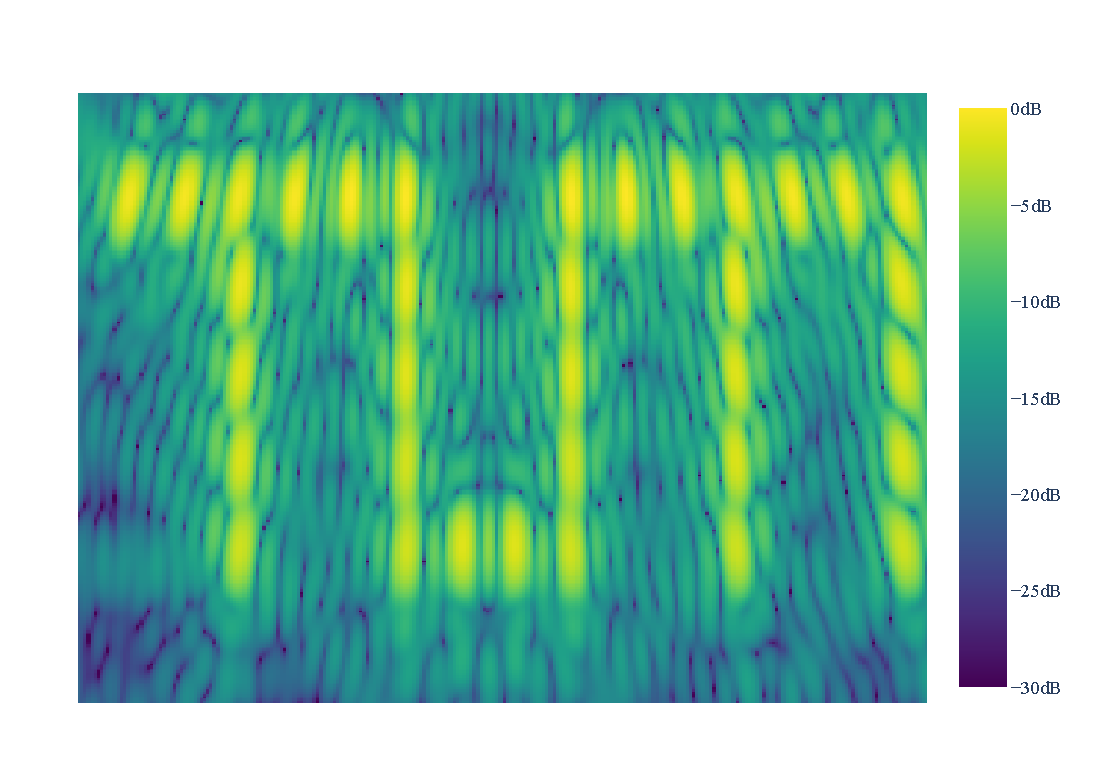
\includegraphics[page=1, width=0.49\textwidth]{figures/pure_los.pdf}
    \caption{The image of the pure LOS-scenario}\label{fig:los_results}
\end{figure}

The calculated image for this scenario is shown in Figure~\ref{fig:los_results}.
The emitting dipole sources can be easily localized.
This image would also result from evaluating Equation~\eqref{eq:naive_algorithm} at every point in the imaging domain and coloring the imaging point accordingly.
To do this no knowledge about the medium or the setup is needed and only the distances between the receivers and the imaging points are considered.
This approach is called the naive algorithm.


\section{Pure Non-Line-of-Sight (NLOS) Scenarios}
To create a pure Non-Line-of-Sight scenario, a PEC-plate is placed between the source and the receiver to block the direct path.
Another PEC-plate is placed perpendicular on top of the blocking plate with a small gap between both plates to create a reflecting path.
The resulting setup is shown in Figure~\ref{fig:nlos_setup}.

\begin{figure}[p]
    \centering
    \includegraphics[trim=0 0 0 70pt, clip, page=3, width=0.8\textwidth]{figures/pure_nlos.pdf}
    \caption{The NLOS Setup}\label{fig:nlos_setup}

    \includegraphics[page=2, width=0.49\textwidth]{figures/pure_nlos_naive.pdf}
    \includegraphics[page=2, width=0.49\textwidth]{figures/pure_nlos.pdf}
    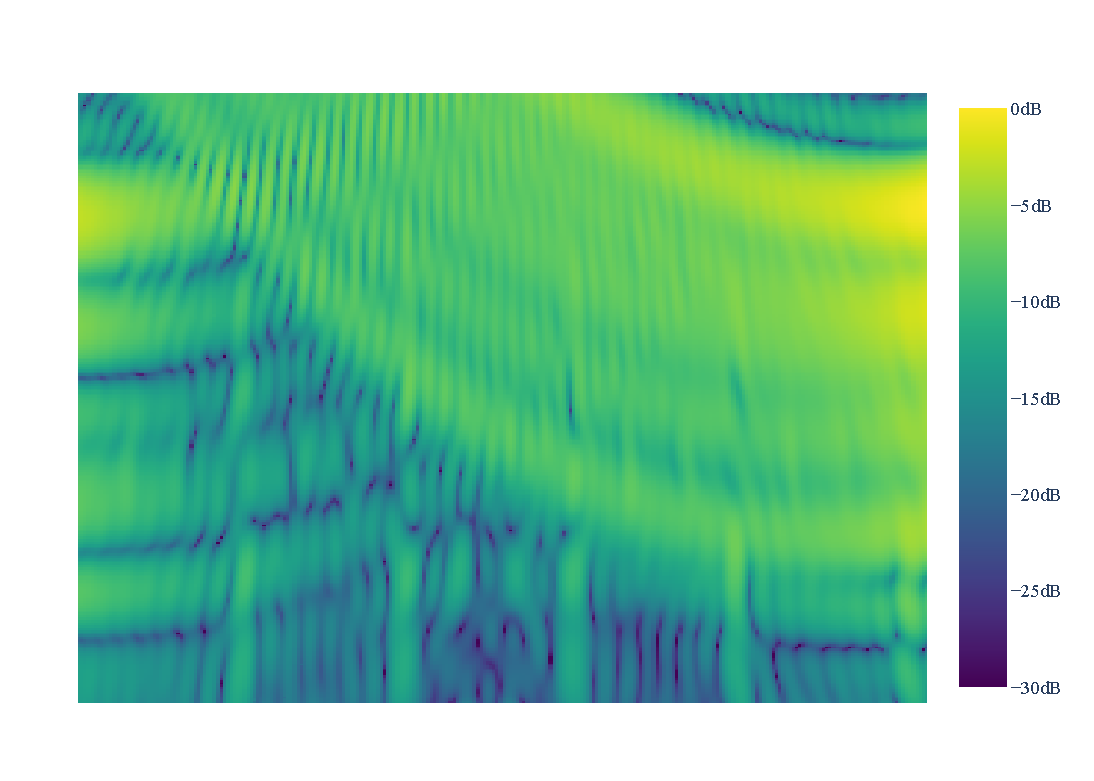
\includegraphics[page=1, width=0.49\textwidth]{figures/pure_nlos_naive.pdf}
    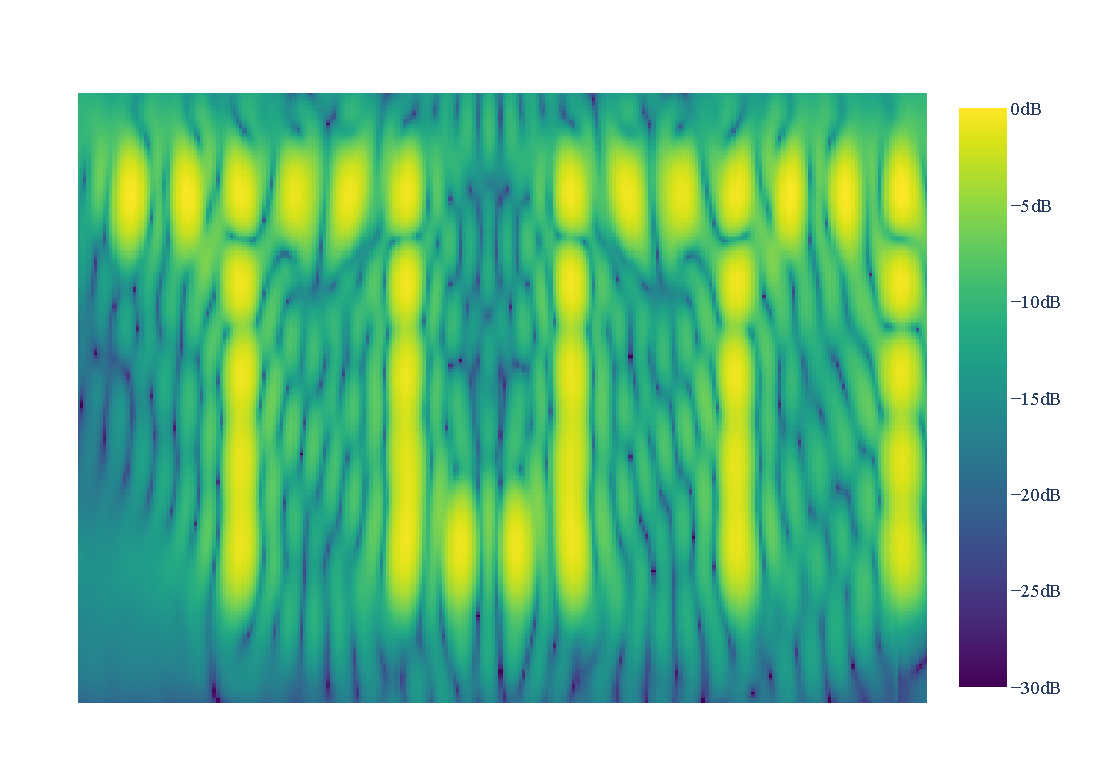
\includegraphics[page=1, width=0.49\textwidth]{figures/pure_nlos.pdf}
    \caption{The Intensity of the Backpropagated field using a naive algorithm (left) compared to the ray-tracing algorithm (right)}\label{fig:nlos_results}
\end{figure}

In this setup only a small fraction of the emitted wave passes through the gap, reflect off the top plate and reach the receivers.
A simpler algorithm that only considers the distances between the receivers and the imaging points would fail to reconstruct the dipole locations.
The proposed algorithm on the other hand is able to reconstruct the sources as shown in Figure~\ref{fig:nlos_results}.
In the plots the paths of the rays that are considered by the algorithm are visualized as yellow lines for some of the imaging points.
This scenario with only one reflection off a plane PEC-plate is very similar to the pure LOS-scenario.
There is no multipath propagation between the source and the receiver, so the algorithm can be simplified to a similar form as Equation~\eqref{eq:naive_algorithm} with the only difference being that the distance between the imaging point and the \textbf{mirrored} receiver-location should be considered.



\section{Multipath Scenarios}
The initial idea for using the ray-tracing algorithm is to improve the imaging for multipath scenarios.
The resulting image should theoretically enhance if the geometry of the setup and therefore all the paths between the imaging domain and receivers are taken into account, as more information is available than in a naive approach.
To test this, the following two scenarios are considered (see Figure~\ref{fig:MultipathNLOS_setup}).
First a setup with multiple reflecting paths and a direct path between the source and the receiver is examined (LOS).
To create the reflecting paths, a room made of PEC-plates is constructed around the setup.
This room is is only open to the side where the receivers are placed, so most of the energy of the sources is guided to them.
Secondly the same setup is used, but a blocking plate is placed in front of the dipoles, so no direct path between the source and the receiver exists (NLOS).

\begin{figure}[ht]
    \centering
    \includegraphics[page=3, width=0.49\textwidth]{figures/multipath_los_combined.pdf}
    \includegraphics[page=3, width=0.49\textwidth]{figures/multipath_nlos_combined.pdf}
    \caption{The Multipath Setup for LOS (left) and NLOS (right)}\label{fig:MultipathNLOS_setup}
\end{figure}

\subsection{LOS Multipath}
The expectation for the LOS Multipath scenario is, that the source-locations is mostly reconstructed by the direct LOS wavefront.
However there should be noise in the image due to the multipath propagation off the walls.
The question is, whether considering the paths of the other wavefronts actually improves the image quality.
As can be seen in Figure~\ref{fig:MultipathLOS}, both images are a very good approximation of the source-locations.
A closer look reveals that in the image where only the direct wavefront is considered, the dipoles closer to the receivers are shown more intensely than the dipoles further away.
The right image shows almost the same intensity for all dipoles, which is the expected result.
Furthermore the image quality is slightly better when all the wavefronts are considered, as the sources appear much sharper.

\begin{figure}[ht]
    \centering
    \includegraphics[page=2, width=0.49\textwidth]{figures/multipath_los_direct.pdf}
    \includegraphics[page=2, width=0.49\textwidth]{figures/multipath_los_combined.pdf}
    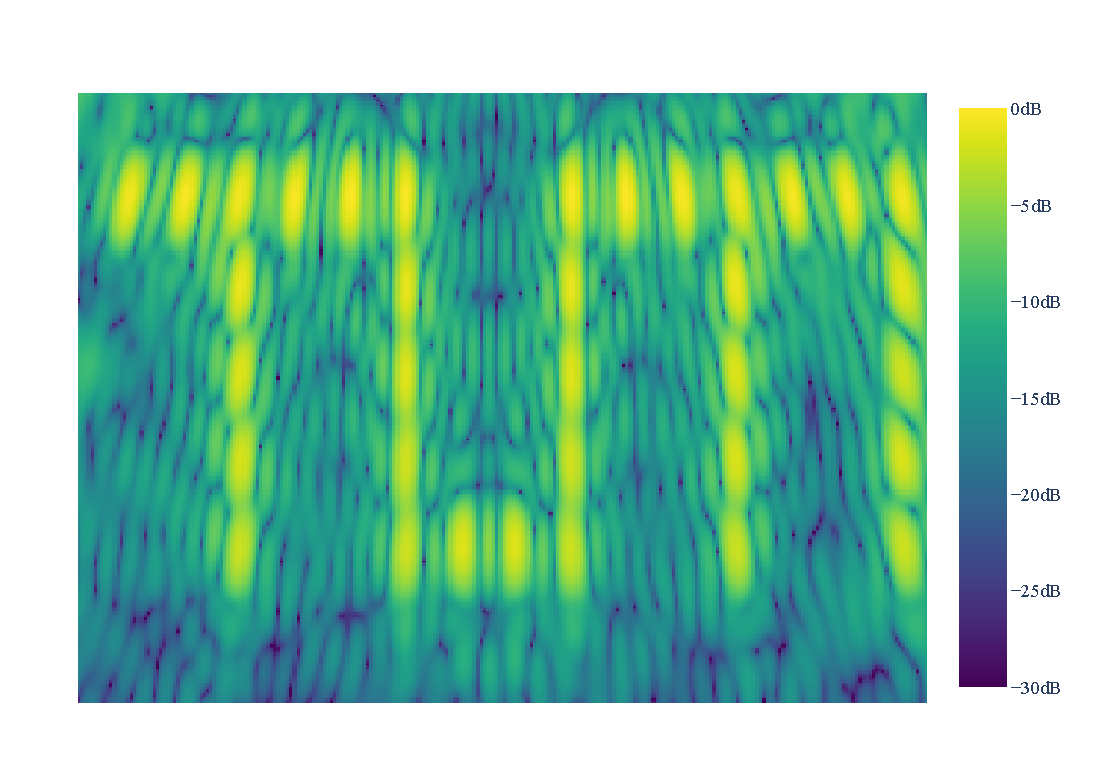
\includegraphics[page=1, width=0.49\textwidth]{figures/multipath_los_direct.pdf}
    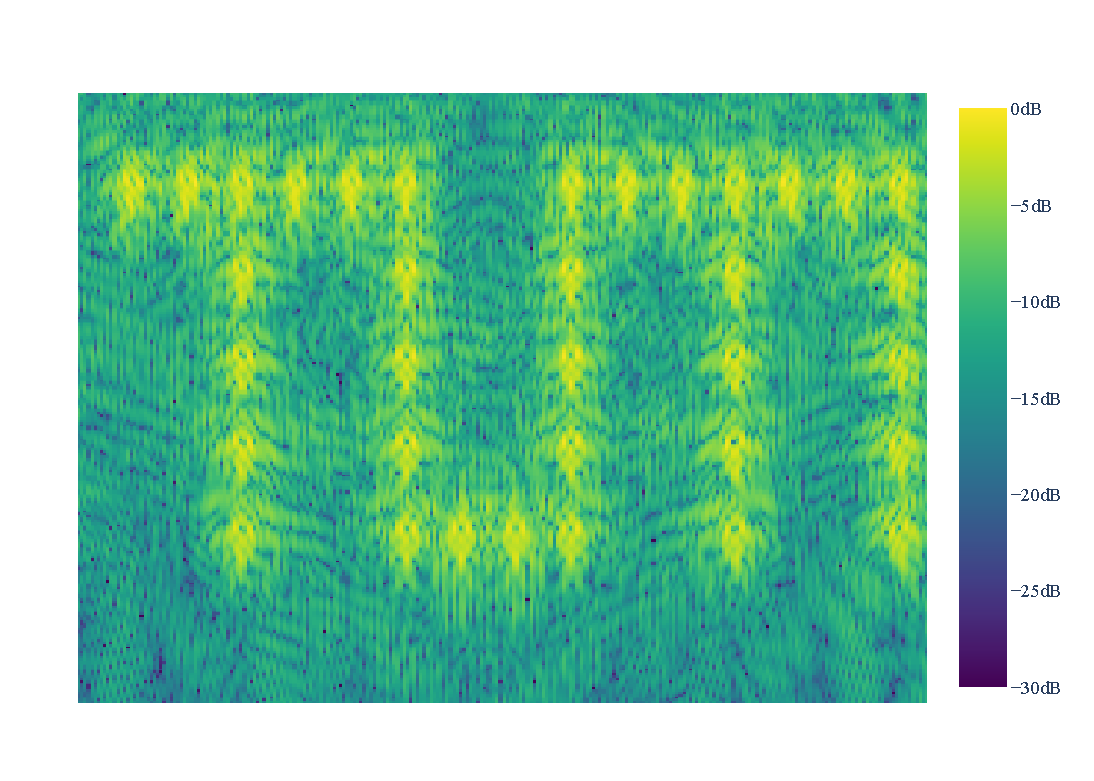
\includegraphics[page=1, width=0.49\textwidth]{figures/multipath_los_combined.pdf}
    \caption{The LOS-results considering only the direct wavefront (left) and combining all wavefronts (right)}\label{fig:MultipathLOS}
\end{figure}

\subsection{NLOS Multipath}
In this multipath setup no LOS-wavefront exists, so the image can only be reconstructed by the reflected wavefronts.
To show, that the algorithm actually improves by considering all the paths, the image for every wavefront is compared to their combined result which is retrieved by summing up the images of every wavefront.
The results for each single wavefront in the NLOS Multipath scenario are shown in Figure~\ref{fig:MultipathNLOS_results}.
They all indicate information about parts of the imaging domain, but none can be used alone to reconstruct the source-locations.
The combined image however shows the dipoles clearly with just a little inaccuracy directly behind the blocking wall (see Figure~\ref{fig:MultipathNLOS_combined}).
This can be explained by the fact that in this area two of the four wavefronts do not contribute any information as indicated by the blue shadow in their individual images.
To solve this problem, the room around the setting could be improved, so there are multiple reflecting paths to every point in the imaging domain.

\begin{figure}[ht]
    \centering
    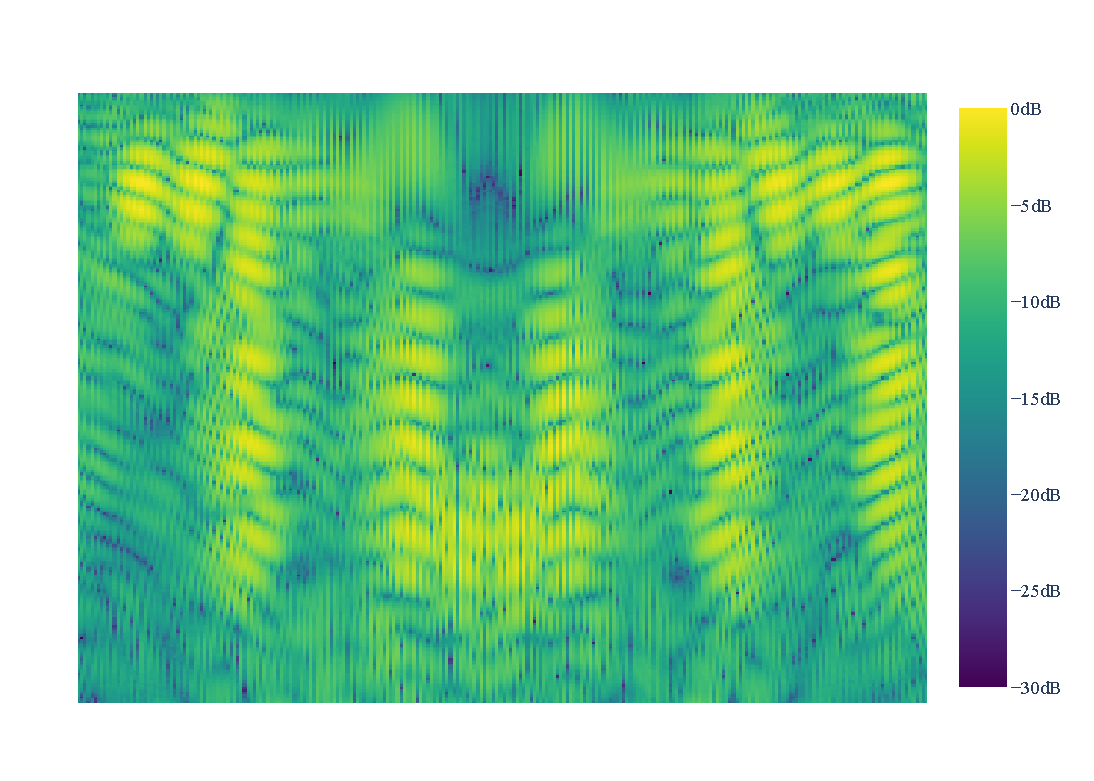
\includegraphics[page=1, width=0.7\textwidth]{figures/multipath_nlos_combined.pdf}
    \caption{The combined image of all the single wavefronts together}\label{fig:MultipathNLOS_combined}
\end{figure}

\begin{figure}[hp]
    \centering
    \vspace{-1.5em} % Adjust this value to reduce the gap
    \includegraphics[page=2, trim=0mm 10mm 0mm 20mm, clip, width=0.49\textwidth]{figures/multipath_nlos_wavefront1.pdf}
    \includegraphics[page=2, trim=0mm 10mm 0mm 20mm, clip, width=0.49\textwidth]{figures/multipath_nlos_wavefront2.pdf}
    \vspace{-1em} % Adjust this value to reduce the gap
    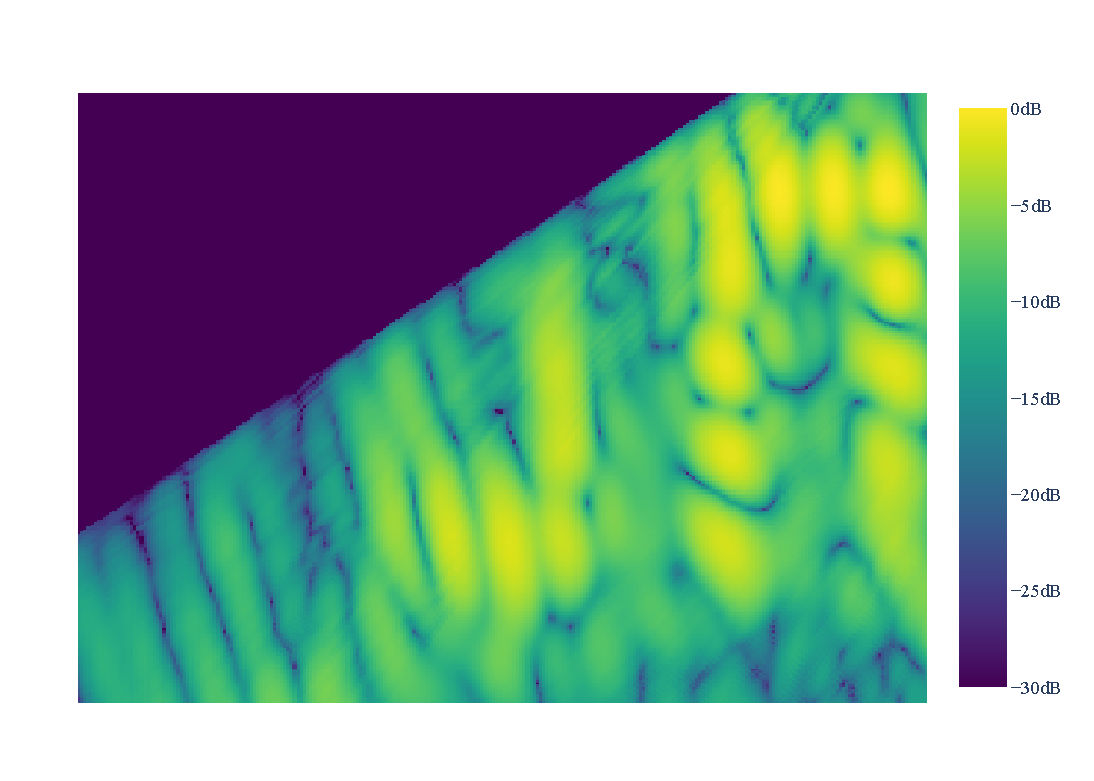
\includegraphics[page=1, width=0.49\textwidth]{figures/multipath_nlos_wavefront1.pdf}
    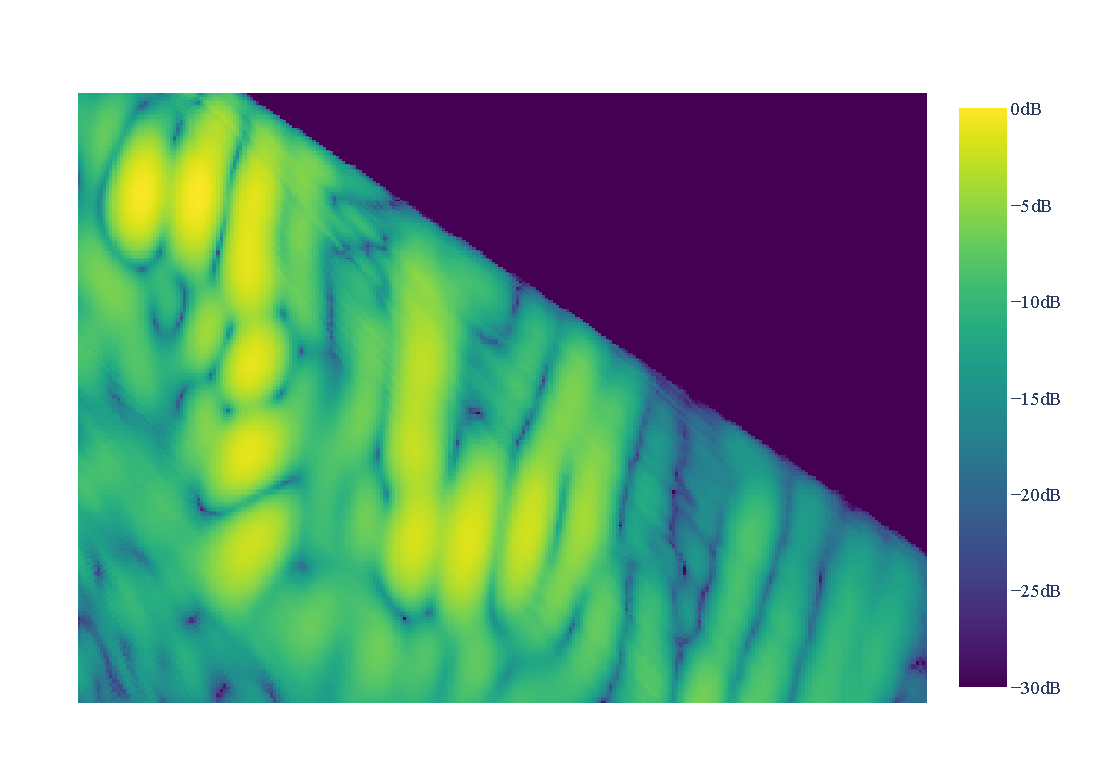
\includegraphics[page=1, width=0.49\textwidth]{figures/multipath_nlos_wavefront2.pdf}
    \vspace{-1em} % Adjust this value to reduce the gap
    \includegraphics[page=2, trim=0mm 10mm 0mm 20mm, clip, width=0.49\textwidth]{figures/multipath_nlos_wavefront3.pdf}
    \includegraphics[page=2, trim=0mm 10mm 0mm 20mm, clip, width=0.49\textwidth]{figures/multipath_nlos_wavefront4.pdf}
    \vspace{-1em} % Adjust this value to reduce the gap
    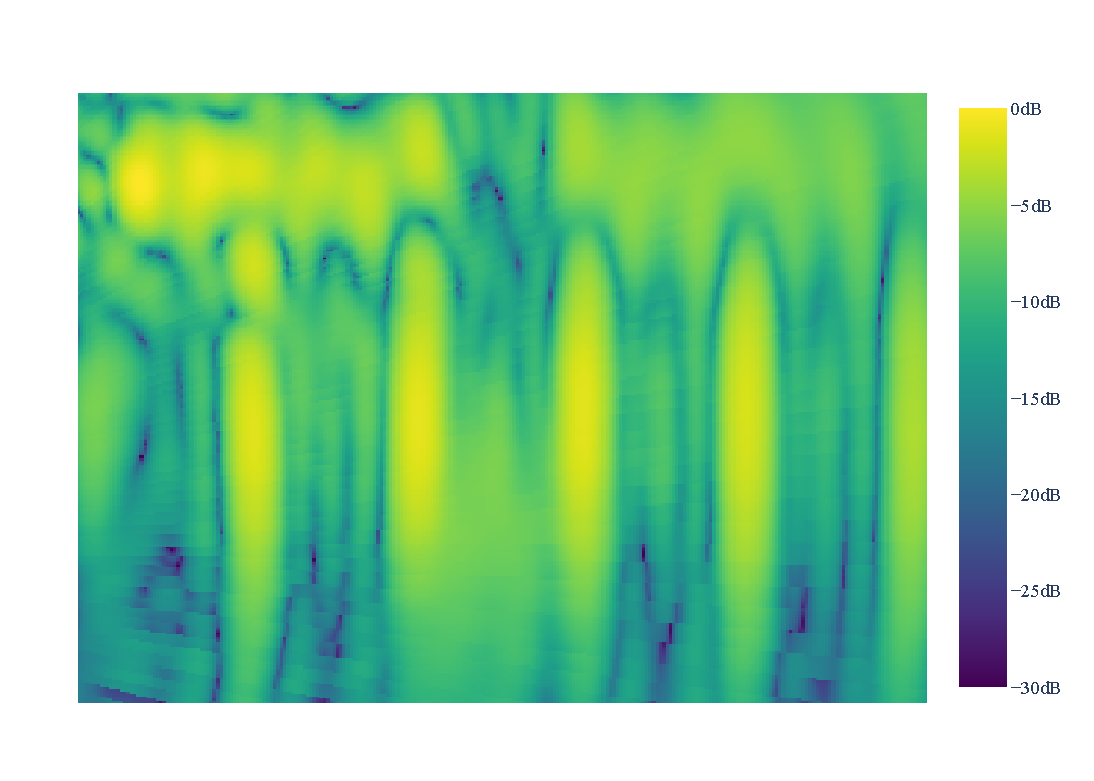
\includegraphics[page=1, width=0.49\textwidth]{figures/multipath_nlos_wavefront3.pdf}
    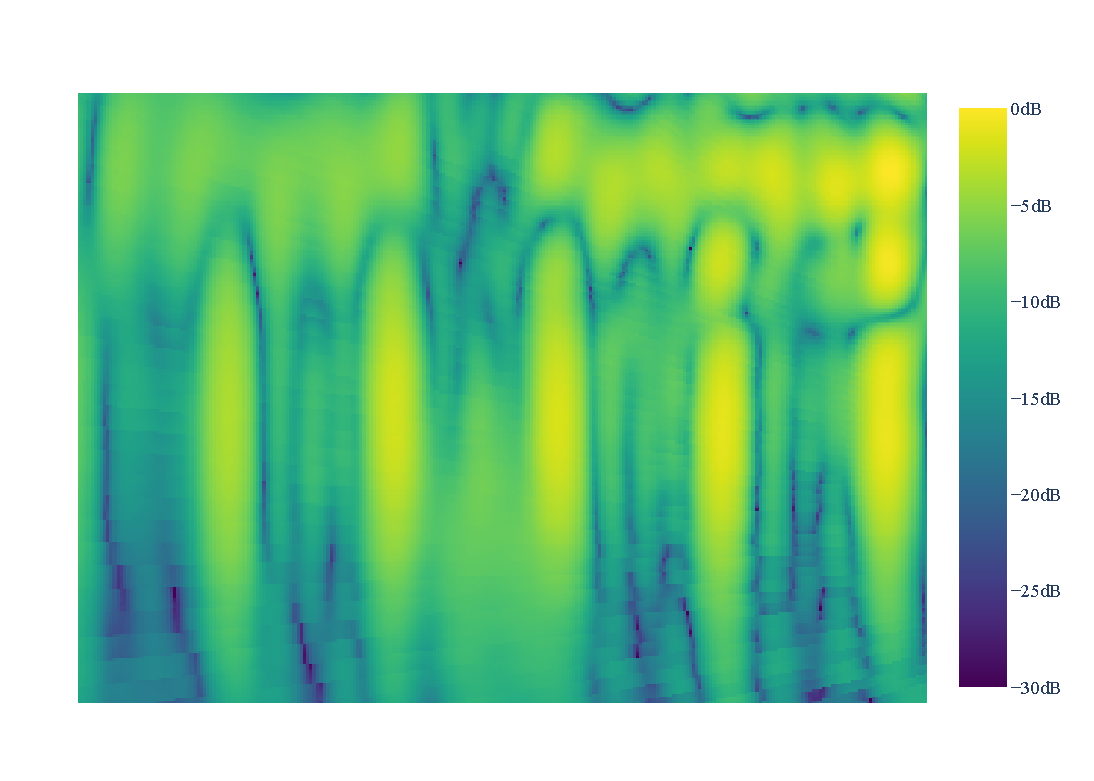
\includegraphics[page=1, width=0.49\textwidth]{figures/multipath_nlos_wavefront4.pdf}
    \caption{The resulting images for all four wavefronts in the NLOS-multipath scenario}\label{fig:MultipathNLOS_results}
\end{figure}

\newpage
\section{Limitations and Robustness}
The previous section showed that the presented algorithm works in the specified scenario.
Although the results are quite promising, as it was possible to reconstruct the original sources quite well, there are limitations of the algorithm that should be considered when applying it.
It was shown, that the contribution of NLOS wavefronts is only marginal if there is a direct path between the imaging domain and the receivers.
Despite the fact that they improved the image quality in some sense, in most cases the constructed image from the LOS wavefront would be sufficient.
This is important because every wavefront needs the same computational time to be computed, so a significant amount of time could be saved by only computing the LOS wavefront.

On the other hand the algorithm is generally very robust when it comes to the computational time needed.
As it is executed by a `NVIDIA GeForce GTX 1080' GPU it took only 265 seconds to compute all the wavefronts for the NLOS multipath scenario.
The GPU takes less than five seconds to perform the calculation for one billion rays.
In the mentioned scenario \(100 \cdot 100 = 10000\) receivers had to be connected with \(256 \cdot 256 = 65536\) imaging points, every ray has to be computed for every wavefront and every frequency.
This results in \(10000 \cdot 65536 \cdot 20 \cdot 4 \approx 52\) billion rays.
Taking this huge number into account it is understandable, how the the utilization of the GPU can speed up the computation significantly.
A way to reduce the computational time even further would be considering less frequencies or considering less measured data.
It turns out, that reducing the number of frequencies to five instead of twenty frequencies results in a noticeable worse image quality, but the reduction of receivers to 2500 instead of 10000 still produces good results.

\begin{figure}[h]
    \centering
    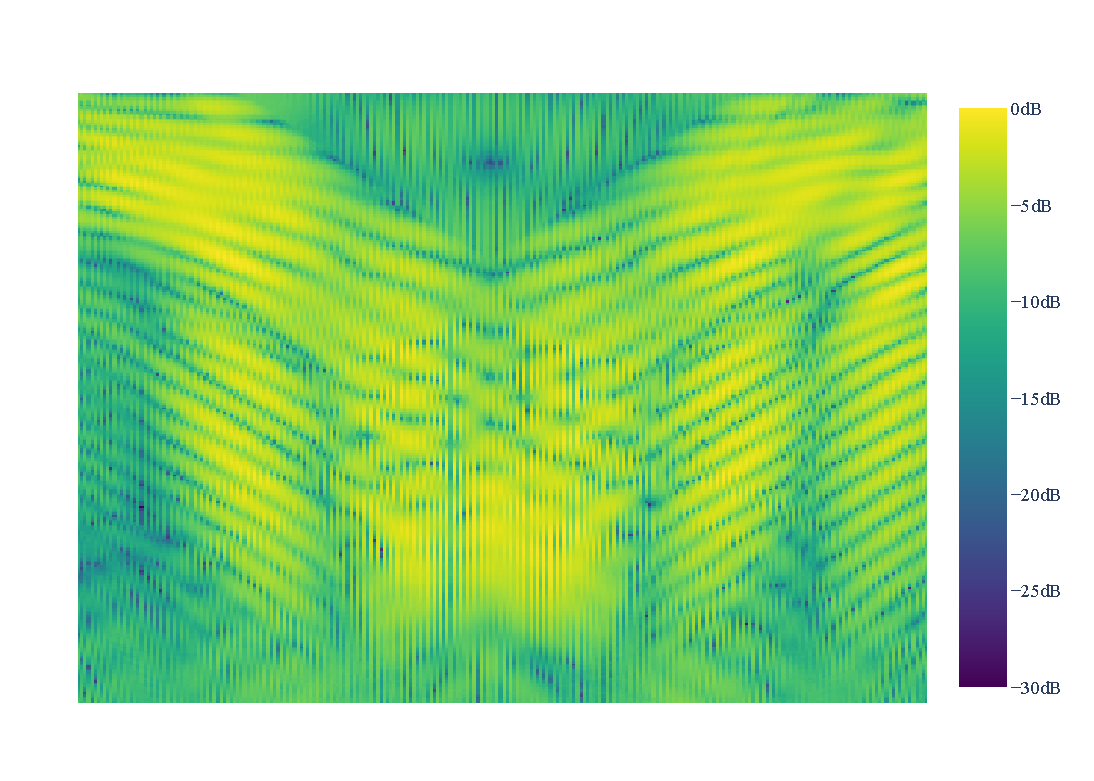
\includegraphics[page=1, width=0.49\textwidth]{figures/multipath_nlos_reduced_freq.pdf}
    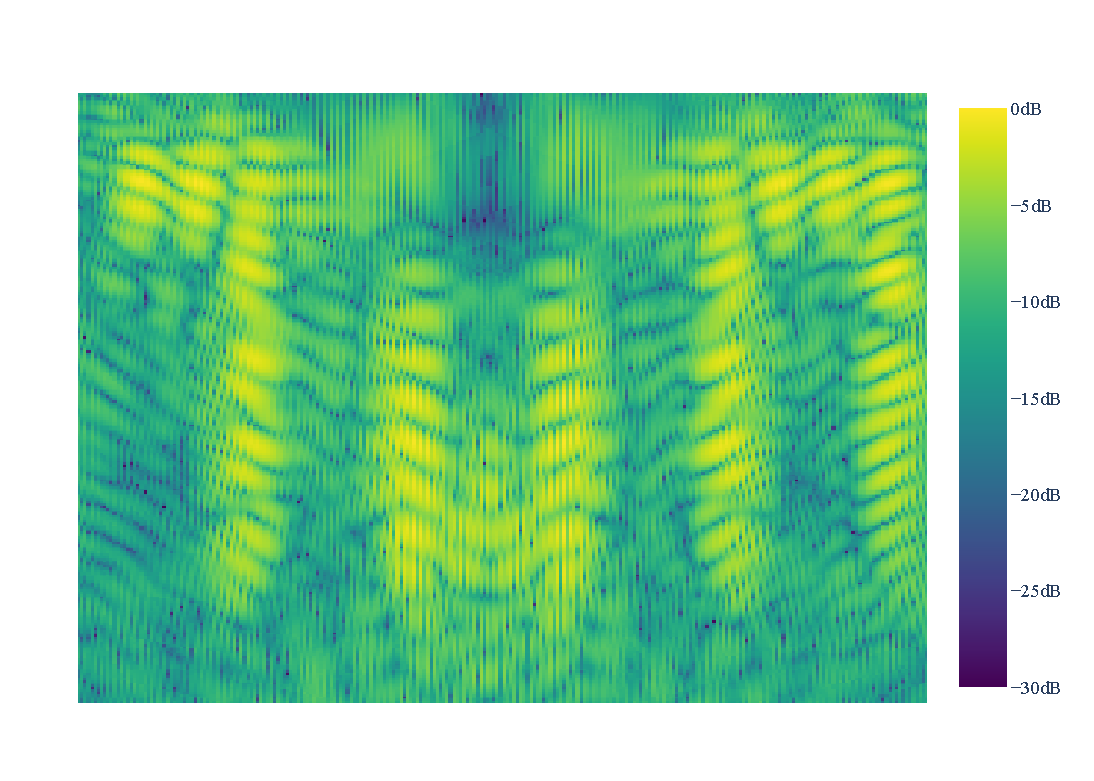
\includegraphics[page=1, width=0.49\textwidth]{figures/multipath_nlos_reduced_receiver.pdf}
    \caption{The results with less frequencies (left) and less receivers (right)}\label{fig:MultipathNLOS_time_optimized}
\end{figure}

